\documentclass[11pt,twoside]{extarticle}
\usepackage{floatrow}   
\usepackage{etex}
%\reserveinserts{18}
\usepackage[english]{babel}
\usepackage{url} % break the too-long url
\def\UrlBreaks{\do\/\do-}
\usepackage[breaklinks]{hyperref}
\usepackage{comment}
 
\usepackage[figuresright]{rotating}
%\newcommand*{\Appendixautorefname}{Appendix} % allowing autoref to show "Appendix"
%\usepackage{xr}  % cross reference
%\externaldocument{Appendix}
\usepackage[margin=1.2in]{geometry}  % margin
\usepackage{setspace}  % single or double spacing
\renewcommand{\baselinestretch}{1.3}
\usepackage{booktabs, multicol}   % \toprule[1.25pt] in Table//.
\usepackage{threeparttable}   % add Table notes
%\usepackage{lscape}
\usepackage{pdflscape}
\usepackage{xcolor}
\usepackage{amstext}
\usepackage{pgfplots}
\usepackage{color}
\usepackage{soul}
\usetikzlibrary{shapes,positioning,matrix,calc,shapes,shapes.multipart,shapes.misc,arrows,chains,fit,plotmarks}
\usetikzlibrary{decorations.text}
%\pgfplotsset{width=23cm,height = 18cm, compat=1.10}

\usepackage{eurosym}
\usepackage{amssymb}
\usepackage{amsfonts}

\usepackage{afterpage}
%Avoid horizontal figure to generate a blank page

\usepackage{epsfig}
\usepackage{upgreek}
\usepackage{commath}
\usepackage{enumitem}
\usepackage{subfigure}
\usepackage{indentfirst}
\usepackage{xr}  
\usepackage{dsfont}
\usepackage{cleveref}
\usepackage{titlesec}
\usepackage{titling}
\usepackage{multibib}
\usepackage{makecell}
\usepackage{soul}
\usepackage{arydshln}
\usepackage{mathrsfs}
\usepackage{ragged2e}
\newcites{online}{References} %% online appendix
% \usepackage{amsfonts}
\allowdisplaybreaks % pagebreak aligned equations

\usepackage[normalem]{ulem} % to highlight changes between versions

\setcounter{MaxMatrixCols}{10}
%TCIDATA{OutputFilter=LATEX.DLL}
%TCIDATA{Version=5.50.0.2953}
%TCIDATA{Codepage=932}
%TCIDATA{<META NAME="SaveForMode" CONTENT="1">}
%TCIDATA{BibliographyScheme=Manual}
%TCIDATA{LastRevised=Saturday, October 22, 2016 13:04:05}
%TCIDATA{<META NAME="GraphicsSave" CONTENT="32">}
%TCIDATA{Language=American English}
%TCIDATA{CSTFile=LaTeX article (bright).cst}

\newtheorem{theorem}{Theorem}
\newtheorem{acknowledgement}{Acknowledgement}
\newtheorem{algorithm}{Algorithm}
\newtheorem{assumption}{Assumption}
\newtheorem{axiom}{Axiom}
\newtheorem{case}{Case}
\newtheorem{claim}{Claim}
\newtheorem{conclusion}{Conclusion}
\newtheorem{condition}{Condition}
\newtheorem{conjecture}{Conjecture}
\newtheorem{corollary}{Corollary}
\newtheorem{criterion}{Criterion}
\newtheorem{definition}{Definition}
\newtheorem{example}{Example}
\newtheorem{observation}{Observation}
\newtheorem{exercise}{Exercise}
\newtheorem{lemma}{Lemma}
\newtheorem{notation}{Notation}
\newtheorem{problem}{Problem}
\newtheorem{proposition}{Proposition}
\newtheorem{remark}{Remark}
\newtheorem{solution}{Solution}
\newtheorem{summary}{Summary}
\providecommand*{\theoremautorefname}{Theorem}
\providecommand*{\lemmaautorefname}{Lemma}
\providecommand*{\propositionautorefname}{Proposition}
\providecommand*{\corollaryautorefname}{Corollary}
\providecommand*{\definitionautorefname}{Definition}
\newenvironment{proof}[1][Proof]{\noindent \textbf{#1.} }{\ \rule{0.5em}{0.5em}}
\geometry{left=1.2in,right=1.2in,top=1.3in,bottom=1.3in}
\renewcommand{\baselinestretch}{1.3}
\newcommand{\newln}{\\&\quad\quad{}}
\newcommand{\parenthnewln}{\right.\\&\left.\quad\quad{}}
% \newcommand{\cn}[1]{\citet*{#1}}
% \newcommand{\cnp}[1]{(\citealt{#1})}  % (Jones 2002)
\usepackage{bbm}

\usepackage{longtable}
\usepackage[para]{threeparttablex} % for "ThreePartTable" environment

\usepackage{float}
\usepackage[titletoc,title]{appendix} % enable appendix environment
\raggedbottom % better manage spaces between paragraphs

\usepackage{amsmath}
\usepackage{bm}
\usepackage{lineno} % add line number to pdf

\usepackage[T1]{fontenc}
\usepackage{palatino}

\usepackage{graphicx}

\hypersetup{
   colorlinks=true,linkcolor=blue,citecolor=blue, filecolor=magenta, citebordercolor=yellow,
   linkbordercolor = magenta
}

\usepackage{graphicx}
\usepackage{subfigure}
\floatsetup[figure]{font=footnotesize}

\floatsetup[table]{capposition=top} % Table title at the top
\floatsetup[table]{font=footnotesize}

\floatsetup{style=plain,footposition=bottom}
\floatsetup[figure]{capposition=bottom}

\usepackage{multirow} % multiple lines per cell
\newcommand{\specialcell}[2][c]{% \specialcell[t]{} % aligned with top rule
        \begin{tabular}[#1]{@{}c@{}}#2\end{tabular}}

\makeatletter
\renewcommand\@makefntext[1]{% footnoot 1. style
    \parindent 1em%
    \@thefnmark.~#1$\qquad$}
\makeatother

\usepackage{tabularx}
\newcolumntype{R}{>{\raggedleft\arraybackslash}X}
\newcolumntype{L}{>{\raggedright\arraybackslash}X}
\newcolumntype{C}{>{\centering\arraybackslash}X}

\usepackage[figuresright]{rotating}

% caption styling
\usepackage[font=normalsize,format=plain,labelfont=bf,up,textfont=up,justification=centering]{caption}
\captionsetup[table]{labelsep=space}   % no : in caption
\captionsetup[figure]{labelsep=space}
\addto\captionsenglish{%
\renewcommand{\figurename}{FIGURE}
\renewcommand{\tablename}{TABLE}}
\renewcommand{\thesubfigure}{(\Alph{subfigure})} 

\usepackage{natbib} % references author-year display
\newcommand{\cites}[1]{\citeauthor{#1}'s (\citeyear{#1})} % author's (2010) style

\usepackage{pdflscape} % \begin{landscape}
\newcommand{\jw}[1]{\textcolor{cyan}{[JW: #1]}}
\newcommand{\yy}[1]{\textcolor{orange}{[YY: #1]}}
\newcommand{\zz}[1]{\textcolor{red}{[ZZ: #1]}}

\usepackage[titletoc]{appendix}
\usepackage{titletoc}

\title{Manufacturing Enemies in Political Contests}
\author{Haotian (George) Bai\thanks{I thank to conference/seminar participants at xxx. I extend special thank to Prof. Jean-Paul Carvalho (Oxford).}}
\date{\today}

\begin{document}

\maketitle

\begin{abstract}

\begin{center}
    \textcolor{red}{This is model abstract only (to provide an outline for the model part). Motivating facts to be finished. I will put the reduced-form motivating evidence before the model.}
\end{center}
\vspace{0.3cm}
Two Majority parties compete for office: a \emph{Dove} with a comparative advantage in economic public good provision and a \emph{Hawk} with superior security technology (state capacity). Security is micro-founded as a Tullock contest between decentralized Majority enforcement and Minority mobilization. In peaceful environments, minority mobilization is absent, the contest is dormant, and realized security is high under either party; elections then hinge on economic performance, where the Hawk is disadvantaged. I show that the Hawk can overturn this by choosing provocative symbolic policy ($d>0$) that manufactures a visible threat and triggers Minority mobilization. The induced threat activates the security dimension by relaxing Majority free-riding and raising decentralized enforcement, so the Hawk's superior state capacity translates into a Security Premium at the ballot box. Symbolic provocation is therefore an electoral substitute for economic competence, but it is disciplined: beyond a peak threat level, additional mobilization discourages Majority enforcement, so further provocation yields diminishing electoral returns while raising direct policy costs. The mechanism implies strictly positive rent dissipation whenever provocation is used. A dynamic extension with noisy performance signals and stochastic shocks clarifies long-run political outcomes. With patient, forward-looking voters, the Hawk becomes an absorbing conflict-trap regime despite economic underperformance; with myopic retrospective voters, the polity exhibits political cycles, oscillating between Dove regimes and Hawk regimes.
\end{abstract}

\section{The Model Environment}

Consider an economy populated by a measure one continuum of citizens divided into two distinct ethnic or religious groups: a Majority $M$ and a Minority $m$. The Majority comprises a population share $n_M > 1/2$, while the Minority comprises the remainder $n_m = 1 - n_M$. The Majority group is represented by two competing political parties, Party $A$ (the \emph{Hawk}) and Party $B$ (the \emph{Dove}), who compete for the electoral support of the Majority representative voter.

The incumbent party $k \in \{A, B\}$ selects a policy vector $\mathbf{q}_k = (d_k, g_k) \in \mathbb{R}_+^2$ subject to their technological constraints. The policy consists of two instruments. First, the symbolic policy $d$ represents the intensity of identity-based regulations, such as cultural bans or dress codes, which serve as a coordination device for identity grievances. Second, economic policy $g$ captures the provision of public policies on public goods provision, market integration, or employment opportunities.

Parties are distinguished by their technological capabilities in delivering these policies. We assume that Party $A$ possesses a comparative advantage in the production of security and coercion, denoted by competence parameter $S_A$. Conversely, Party $B$ possesses a comparative advantage in economic management but holds inferior security competence $S_B$. Formally, we posit that $S_A > S_B$, while the cost of providing public goods satisfies $c_A(g) > c_B(g)$ for any equivalent level of $g$.

\subsection*{Timing and solution concept}
The political interaction is a three-stage game solved by backward induction.
\begin{enumerate}[label=\textbf{Stage \arabic*:}, leftmargin=*, itemsep=0.2em]
    \item \textbf{Policy choice.} The incumbent party $k\in\{A,B\}$ selects a policy vector $(d_k,g_k)$.
    \item \textbf{Contest and mobilization.} Given the symbolic environment induced by $d_k$, the Minority mobilizes, and Majority citizens choose enforcement effort given the incumbent's security competence $S_k$.
    \item \textbf{Election.} The Majority electorate votes between the Hawk and the Dove. In a stationary equilibrium, voters evaluate each party using the equilibrium outcomes implied by backward induction.
\end{enumerate}

The equilibrium concept is subgame perfect equilibrium. In the contest subgame among Majority citizens, I focus on symmetric Nash equilibria. The key strategic margin is the choice of $d_k$: the economic gap $u(g_B)-u(g_A)$ is treated as a reduced-form party characteristic, while the model endogenizes how symbolic policy changes the security advantage associated with $S_A>S_B$.

\section{Micro-foundations of Conflict and Collective Action}

Conflict in this economy is modeled as a contest over political dominance. Unlike standard contest models where groups act as unitary actors, I explicitly model the collective action problem within each group.

\subsection{The Minority's Reaction}
Minority mobilization is an endogenous response to the grievance generated by symbolic policy. The representative minority member chooses effort to minimize the loss from symbolic oppression net of effort costs.

Formally, the representative agent chooses effort level $e_m$ to maximize a utility function $V(e_m; d)$. This function balances the psychological gratification of resistance against the convex cost of mobilization:
\begin{equation}
    \max_{e_m \geq 0} \quad V(e_m; d) = \underbrace{\phi d^{\sigma} e_m}_{\text{Expressive Utility}} - \underbrace{\frac{1}{2\kappa} e_m^2}_{\text{Cost of Effort}}
\end{equation}
The first term captures the marginal benefit of resistance, where $\phi > 0$ represents the group's \textit{sensitivity to grievance} and $d^\sigma$ captures the intensity of the symbolic shock (with elasticity $\sigma > 0$). The second term represents the cost of mobilization, where $\kappa > 0$ denotes the group's \textit{organizational capacity} (or social capital). A higher $\kappa$ reduces the marginal cost of effort, reflecting stronger internal coordination networks.

The first-order condition (FOC) for an interior solution implies:
\begin{equation}
    \frac{\partial V}{\partial e_m} = \phi d^{\sigma} - \frac{1}{\kappa} e_m = 0.
\end{equation}
Solving for $e_m$, we derive the structural reaction function for aggregate minority mobilization:
\begin{equation} \label{eq:reaction}
    E_m(d) = \gamma d^{\sigma},
\end{equation}
where $\gamma \equiv \phi \kappa$ is the \textit{structural mobilization potential}. This explicit derivation clarifies that the opposition's strength $\gamma$ is a composite of two forces: the intensity of their grievance sensitivity ($\phi$) and their capacity to organize ($\kappa$).


\subsection{The Majority's Collective Action Problem}


While both economic stability and security are public goods, they differ in their production technology. Economic goods are provided top-down by the state, whereas security (dominance) requires decentralized participation by Majority citizens. This creates a standard free-rider problem: each Majority citizen benefits from dominance, but individually underprovides enforcement effort.

Fix an incumbent party $k$ and suppose the Majority consists of $N_M$ identical citizens indexed by $i=1,\dots,N_M$. Citizen $i$ chooses enforcement effort $e_i\ge 0$ at private cost $\frac{1}{2}e_i^2$. Aggregate Majority effort is $E_M\equiv\sum_{j=1}^{N_M} e_j$. Minority mobilization $E_m$ is determined by \autoref{eq:reaction} following the symbolic policy choice.

Security is produced by a stochastic contest between a state-amplified Majority and an oppositional Minority. Let $S_k>0$ denote the incumbent's security competence, which acts as a force multiplier on Majority effort. Following standard contest theory, the probability that the Majority prevails is given by the Tullock contest success function\footnote{Following the contest theory literature (e.g., \citet{skaperdas1996contest}; \citet{jia2008stochastic}), one micro-foundation assumes realized ``performance'' levels $Y_M=\ln(S_k E_M)+\varepsilon_M$ and $Y_m=\ln(E_m)+\varepsilon_m$, where $\varepsilon_M,\varepsilon_m$ are i.i.d.\ Type I Extreme Value (Gumbel). The probability of Majority dominance is $\Pi_k=\mathbb{P}(Y_M>Y_m)$, which simplifies to \autoref{eq:CSF}.}:
\begin{equation} \label{eq:CSF}
\Pi_k(E_M, E_m) = \frac{S_k E_M}{S_k E_M + E_m}.
\end{equation}

This formulation captures the model's central asymmetry: holding office grants access to $S_k$, which scales the effectiveness of decentralized Majority effort, and therefore makes security competence electorally salient when the opposition is mobilized.

Given $(S_k,E_m)$, each Majority citizen $i$ chooses $e_i$ to maximize private utility,
\begin{equation} \label{eq:majority_prob}
    \max_{e_i \geq 0} \quad W_i = \underbrace{\Lambda \cdot \Pi_k(E_{M}, E_m)}_{\text{Public Benefit}} - \underbrace{\frac{1}{2} e_i^2}_{\text{Private Cost}}
\end{equation}
where $\Lambda>0$ is the per-capita valuation of security. Taking aggregate effort of other citizens as given, the first-order condition for an interior best response is
\begin{equation} \label{eq:majority_foc}
e_i = \Lambda \frac{\partial \Pi_k}{\partial E_M}(E_M, E_m)=\Lambda\frac{S_k E_m}{(S_k E_M + E_m)^2}.
\end{equation}
In a symmetric Nash equilibrium, $e_i=e$ for all $i$, so $E_M=N_M e$ and aggregate Majority mobilization $E_M^*(S_k,E_m)$ satisfies
\begin{equation} \label{eq:EM_star}
\frac{E_M^*(S_k,E_m)}{N_M}=\Lambda\frac{S_k E_m}{(S_k E_M^*(S_k,E_m)+E_m)^2}.
\end{equation}

\begin{lemma}[\textbf{Contest equilibrium}] \label{lem:contest_equilibrium}
For any $(S_k,E_m)\in(0,\infty)\times[0,\infty)$, the Majority mobilization game admits a unique symmetric Nash equilibrium. If $E_m=0$, then $E_M^*(S_k,0)=0$. If $E_m>0$, then $E_M^*(S_k,E_m)>0$ is the unique solution to \autoref{eq:EM_star}. Define equilibrium security
\begin{equation} \label{eq:Pi_star}
\Pi_k^*(S_k,E_m)\;\equiv\;\Pi_k\big(E_M^*(S_k,E_m),E_m\big).
\end{equation}
Then $\Pi_k^*(S_k,E_m)$ is strictly increasing in $S_k$ for any $E_m>0$, satisfies $\lim_{E_m\downarrow 0}\Pi_k^*(S_k,E_m)=1$, and satisfies $\lim_{E_m\uparrow\infty}\Pi_k^*(S_k,E_m)=0$.
Security competence is electorally relevant only when the opposition is mobilized: if $E_m=0$ then $\Pi_k^*=1$ under either party, while for any $E_m>0$ higher $S_k$ delivers higher equilibrium security.
\end{lemma}

\begin{proof}
If $E_m=0$, then $\Pi_k(E_M,0)=1$ for all $E_M\ge 0$, so the unique best response is $e_i=0$ and hence $E_M^*(S_k,0)=0$.

Fix $E_m>0$ and $S_k>0$. Under symmetry, \autoref{eq:EM_star} is equivalent to
\begin{equation} \label{eq:EM_star_cubic}
\frac{E_M}{N_M}(S_k E_M+E_m)^2=\Lambda S_k E_m.
\end{equation}
Define $f(E_M)\equiv\frac{E_M}{N_M}(S_k E_M+E_m)^2-\Lambda S_k E_m$. The function $f$ is continuous on $[0,\infty)$ with $f(0)=-\Lambda S_k E_m<0$, and
\[
f'(E_M)=\frac{1}{N_M}(S_k E_M+E_m)(3S_k E_M+E_m)>0
\]
for all $E_M\ge 0$. Moreover, $\lim_{E_M\to\infty}f(E_M)=+\infty$. Hence there exists a unique $E_M^*(S_k,E_m)>0$ satisfying \autoref{eq:EM_star_cubic}.

To establish monotonicity in $S_k$, define effective enforcement $Z_k\equiv S_k E_M^*(S_k,E_m)$ and rewrite \autoref{eq:EM_star_cubic} as
\begin{equation} \label{eq:Z_star}
Z_k(Z_k+E_m)^2=N_M\Lambda S_k^2 E_m.
\end{equation}
For any fixed $E_m>0$, the left-hand side is strictly increasing in $Z_k$, while the right-hand side is strictly increasing in $S_k^2$. Therefore $Z_k$ is strictly increasing in $S_k$. Since $\Pi_k^*(S_k,E_m)=Z_k/(Z_k+E_m)$ is strictly increasing in $Z_k$, it follows that $\Pi_k^*$ is strictly increasing in $S_k$.

Finally, let $r_k\equiv Z_k/E_m$. Dividing \autoref{eq:Z_star} by $E_m^3$ yields $r_k(r_k+1)^2=N_M\Lambda S_k^2/E_m^2$. As $E_m\downarrow 0$, the right-hand side diverges to $+\infty$, so $r_k\to+\infty$ and hence $\Pi_k^*(S_k,E_m)=r_k/(r_k+1)\to 1$. As $E_m\uparrow\infty$, the right-hand side converges to $0$, so $r_k\to 0$ and hence $\Pi_k^*(S_k,E_m)\to 0$.
\end{proof}

Lemma \autoref{lem:contest_equilibrium} demonstrates that the state capacity is not self-activating. In the contest subgame, enforcement is a decentralized public input, so the Majority faces a grassroots free-rider problem. When the Minority does not mobilize ($E_m=0$), each citizen's marginal impact on dominance is 0 and equilibrium enforcement collapses to 0. However, once $E_m>0$, individual enforcement becomes pivotal at the margin, and higher security competence $S_k$ scales each unit of citizen effort into effective enforcement $Z_k=S_kE_M$, raising the private return to mobilization and making collective action sustainable. Therefore, $S_A$ can be seen as an organizational technology that converts diffuse preferences for order into coordinated street-level effort. Note this technology is dormant in peacetime. When $E_m=0$, both parties deliver full dominance regardless of competence, so the Hawk's advantage becomes electorally invisible. For security competence to have electoral value, a visible Minority threat is a strict structural prerequisite.

Combining \autoref{eq:reaction} and \autoref{eq:Pi_star}, the equilibrium security level under incumbent party $k$ and symbolic policy $d_k$ is
\begin{equation} \label{eq:Pi_star_d}
\Pi_k^*(d_k;S_k)\;\equiv\;\Pi_k^*\big(S_k,E_m(d_k)\big)=\Pi_k^*\big(S_k,\gamma d_k^{\sigma}\big).
\end{equation}
Two implications will be useful below. First, as $d_k\downarrow 0$, minority mobilization vanishes and equilibrium security converges to one under either party. In that limit, differences in security competence are electorally irrelevant because they no longer generate different realized security outcomes. Second, when $d_k>0$ induces a non-trivial threat, higher $S_k$ translates into higher equilibrium security by raising effective enforcement $Z_k$.

\subsection{Manipulating the Group Contest} \label{subsec:contest_theory}

This subsection makes explicit the model's link to contest theory. In canonical contest environments, a (typically neutral) principal designs prizes or rules to shape equilibrium effort and performance (e.g., \citet{barut1998symmetric}). Recent work also emphasizes that increasing the intensity of competition can \emph{discourage} effort, yielding non-monotone response patterns (e.g., \citet{fang2020turning}). In contrast, my political economy environment features a \emph{biased} designer: the incumbent party manipulates the contest \emph{indirectly} through symbolic policy. By choosing $d_k$, the incumbent selects the Minority's equilibrium mobilization $E_m(d_k)$ and thereby the ``threat'' faced in the decentralized Majority subgame. This is the precise sense in which provocative symbolic policy can be interpreted as ``arming the enemy,'' an electoral strategy that increases the intensity of the group contest in order to activate Majority enforcement and magnify the return to security competence.

\subsubsection{Comparative statics on technology $S_k$}
Fix $E_m>0$ and consider how Majority mobilization responds to an increase in state security competence $S_k$. Define
\[
F(E_M,S_k;E_m)\equiv \frac{E_M}{N_M}-\Lambda\frac{S_k E_m}{(S_k E_M+E_m)^2}.
\]
The symmetric equilibrium $E_M^*(S_k,E_m)$ is the unique solution to $F(E_M,S_k;E_m)=0$.

\begin{lemma}[\textbf{State capacity and Majority effort}] \label{lem:Sk_statics}
Fix $E_m>0$. The equilibrium mapping $S_k\mapsto E_M^*(S_k,E_m)$ is continuously differentiable and satisfies
\begin{equation} \label{eq:dEMdS}
\frac{\partial E_M^*(S_k,E_m)}{\partial S_k}
\;=\;
-\frac{\frac{\partial F}{\partial S_k}(E_M^*,S_k;E_m)}{\frac{\partial F}{\partial E_M}(E_M^*,S_k;E_m)}
\;=\;
-\frac{\Lambda E_m\big(S_k E_M^*(S_k,E_m)-E_m\big)}{(S_k E_M^*(S_k,E_m)+E_m)^3\Big[\frac{1}{N_M}+\frac{2\Lambda S_k^2 E_m}{(S_k E_M^*(S_k,E_m)+E_m)^3}\Big]}.
\end{equation}
In particular, $\frac{\partial E_M^*}{\partial S_k}>0$ if and only if $S_k E_M^*(S_k,E_m)<E_m$. Moreover, effective enforcement $Z_k^*(S_k,E_m)\equiv S_k E_M^*(S_k,E_m)$ is strictly increasing in $S_k$.
Higher state capacity raises street-level enforcement when capacity is low relative to the threat, but eventually crowds out citizen effort even as effective enforcement $Z_k^*$ continues to rise.
\end{lemma}

\begin{proof}
Fix $E_m>0$. By Lemma \autoref{lem:contest_equilibrium}, $E_M^*(S_k,E_m)$ is uniquely defined for each $S_k>0$. Moreover,
\[
\frac{\partial F}{\partial E_M}(E_M,S_k;E_m)=\frac{1}{N_M}+\frac{2\Lambda S_k^2 E_m}{(S_k E_M+E_m)^3}>0
\]
for all $E_M\ge 0$ and $S_k>0$, so the Implicit Function Theorem implies that $E_M^*(S_k,E_m)$ is continuously differentiable in $S_k$.

Differentiating $F(E_M^*(S_k,E_m),S_k;E_m)=0$ with respect to $S_k$ yields
\[
\frac{\partial F}{\partial E_M}\frac{\partial E_M^*}{\partial S_k}+\frac{\partial F}{\partial S_k}=0,
\]
where
\[
\frac{\partial F}{\partial S_k}(E_M,S_k;E_m)= -\Lambda E_m\frac{\partial}{\partial S_k}\Big(\frac{S_k}{(S_k E_M+E_m)^2}\Big)
=\Lambda E_m\frac{S_k E_M-E_m}{(S_k E_M+E_m)^3}.
\]
Substituting into the total derivative expression yields \autoref{eq:dEMdS} and the sign characterization.

The final claim follows from Lemma \autoref{lem:contest_equilibrium}, which shows that $Z_k^*(S_k,E_m)$ is strictly increasing in $S_k$ and that $\Pi_k^*(S_k,E_m)=Z_k^*/(Z_k^*+E_m)$ is therefore increasing in $S_k$.
\end{proof}

\begin{corollary}[\textbf{A technology threshold}] \label{cor:Sk_threshold}
Fix $E_m>0$ and define $\overline{S}(E_m)\equiv 2E_m/\sqrt{N_M\Lambda}$. Then $E_M^*(S_k,E_m)$ is strictly increasing in $S_k$ for all $S_k\in(0,\overline{S}(E_m))$, strictly decreasing for all $S_k\in(\overline{S}(E_m),\infty)$, and satisfies $E_M^*(\overline{S}(E_m),E_m)=\sqrt{N_M\Lambda}/2$.
Equilibrium Majority mobilization is therefore inverted-U in state capacity, with a unique peak at $S_k=\overline{S}(E_m)$.
\end{corollary}

\begin{proof}
By Lemma \autoref{lem:Sk_statics}, $\partial E_M^*(S_k,E_m)/\partial S_k=0$ if and only if $S_k E_M^*(S_k,E_m)=E_m$. Substituting this restriction into \autoref{eq:EM_star} yields $E_M^*/N_M=\Lambda/(4E_M^*)$, so $E_M^*=\sqrt{N_M\Lambda}/2$ at any stationary point. Therefore any stationary point must satisfy $S_k=E_m/E_M^*=2E_m/\sqrt{N_M\Lambda}$, proving the expression for $\overline{S}(E_m)$ and the value at the peak.

To see that the stationary point is unique and is a global maximum, define $r\equiv S_k E_M^*(S_k,E_m)/E_m$. As in the proof of Lemma \autoref{lem:contest_equilibrium}, $r$ satisfies $r(r+1)^2=N_M\Lambda S_k^2/E_m^2$, which is strictly increasing in $S_k$. Hence $r$ crosses one exactly once, and Lemma \autoref{lem:Sk_statics} implies that $\partial E_M^*/\partial S_k$ changes sign exactly once (from positive to negative) at $S_k=\overline{S}(E_m)$.
\end{proof}

Corollary \autoref{cor:Sk_threshold} clarifies why a Hawk regime need not coincide with visibly higher Majority street violence. When $S_k$ is low, decentralized enforcement has little leverage in the contest, so free-riding dominates and mobilization is weak. As $S_k$ rises into an intermediate range, each unit of citizen effort becomes more effective in producing dominance. This raises the private marginal return to participation and increases $E_M^*$. In this region, a Hawk that is stronger than the Dove but not overwhelmingly strong relies on grass-roots enforcement: state capacity complements citizen mobilization rather than replacing it. Once $S_k$ exceeds the threshold $\overline{S}(E_m)$, strong public device in identity security dominates private effort of mobilization. The state's coercive apparatus becomes sufficiently effective that dominance can be maintained with less decentralized effort, so the private return to participation falls and citizens withdraw from mobilizing for collections actions that protects their identity. Aggregate mobilization $E_M^*$ then declines even as effective enforcement $Z_k^*=S_kE_M^*$ and equilibrium security $\Pi_k^*$ continue to rise. Thus only a relatively weaker Hawk induces visible mass participation. A sufficiently strong Hawk secures order from above, through state capacity rather than street-level mobilization. The corollary therefore breaks the linear association between hawkish politics and popular enforcement, as a strong Hawk can suppress disorder precisely by making grassroots voilence unattractive.

\begin{figure}[t]
    \centering
    \subfigure[Majority mobilization peaks at $S_k=\overline{S}(E_m)$.]{
        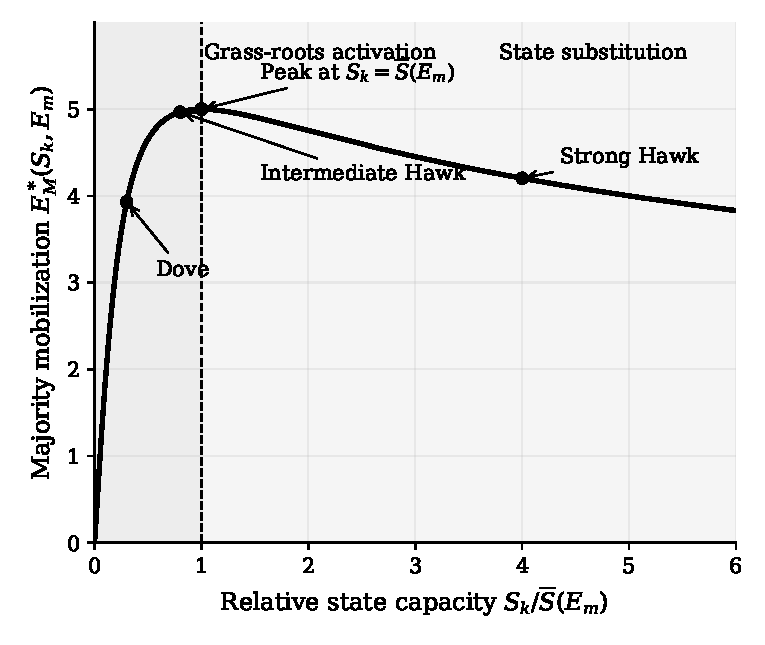
\includegraphics[width=0.46\textwidth]{figures/functions/fig_Sk_statics_mobilization.pdf}
        \label{fig:Sk_statics_mobilization}
    }
    \hfill
    \subfigure[Effective enforcement $Z_k^*$ keeps rising beyond the mobilization peak.]{
        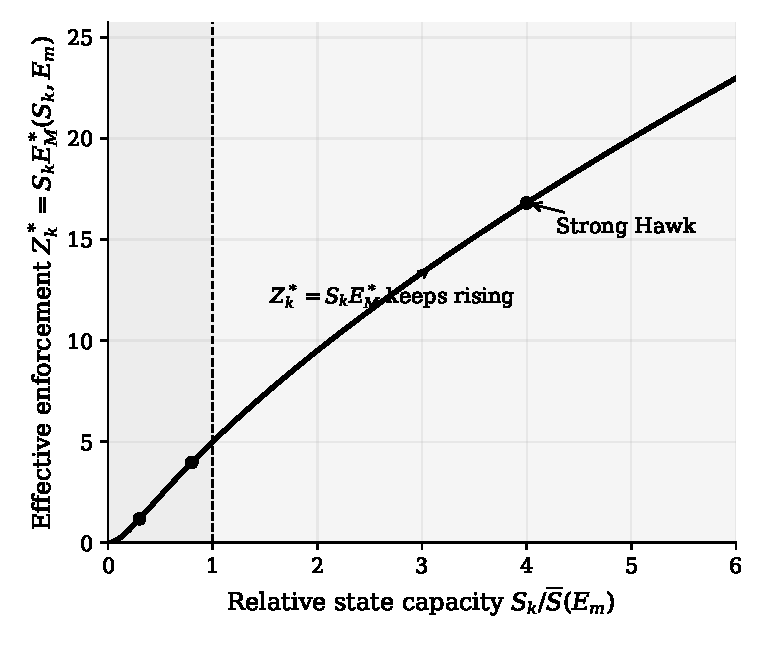
\includegraphics[width=0.46\textwidth]{figures/functions/fig_Sk_statics_enforcement.pdf}
        \label{fig:Sk_statics_enforcement}
    }
    \caption{\normalsize\bf State capacity, street mobilization, and effective enforcement.}
    
    \floatfoot*{\footnotesize\textit{Notes}: The left subfigure plots the symmetric equilibrium $E_M^*(S_k,E_m)$ implied by \autoref{eq:EM_star} against relative state capacity $S_k/\overline{S}(E_m)$, where $\overline{S}(E_m)=2E_m/\sqrt{N_M\Lambda}$ is the threshold from Corollary \autoref{cor:Sk_threshold}. To the left of the threshold, higher state capacity raises the return to decentralized participation and increases Majority mobilization; to the right, stronger state capacity substitutes for street-level effort and $E_M^*$ declines. The right subfigure plots effective enforcement $Z_k^*=S_kE_M^*(S_k,E_m)$ over the same range. Because $Z_k^*$ keeps rising after the peak in $E_M^*$, higher-capacity regimes can generate more effective control with less visible mass participation. The marked points illustrate a low-capacity Dove, an intermediate-capacity Hawk below the threshold, and a stronger Hawk above the threshold. Parameters are $(N_M,\Lambda,E_m)=(100,1,5)$.
    }

    \label{fig:Sk_statics}
\end{figure}

\subsubsection{Reaction functions and strategic complements/substitutes}
For a fixed incumbent technology $S_k$, \autoref{eq:EM_star} defines an implicit reaction function $E_M^*(S_k,E_m)$ mapping the Minority's mobilization into the Majority's equilibrium enforcement. This reaction is generically non-monotone: small threats discipline free-riding and raise enforcement, whereas sufficiently intense threats can discourage enforcement and reduce $E_M^*$.

The non-monotonicity replicates many results from contest theory (insert citations), but it has a distinct implication here because threat is not primitive. Through \autoref{eq:reaction}, symbolic policy $d$ selects the threat level where $E_m(d)=\gamma d^{\sigma}$. The next lemma is a characterization of the Majority reaction function, and it places an endogenous upper bound on politically useful provocation. Since $E_m(d)$ is strictly increasing in $d$, the threat peak maps into a unique symbolic threshold
\begin{equation} \label{eq:d_peak}
d_k^{\mathrm{peak}} \;\equiv\; \left(\frac{E_m^{\mathrm{peak}}(S_k)}{\gamma}\right)^{1/\sigma}
\;=\;
\left(\frac{S_k\sqrt{N_M\Lambda}}{2\gamma}\right)^{1/\sigma}.
\end{equation}
For $d_k<d_k^{\mathrm{peak}}$, stronger symbolic policy raises Minority mobilization and, through that channel, increases Majority enforcement. For $d_k>d_k^{\mathrm{peak}}$, further provocation is counterproductive: it pushes the economy into the discouragement region, where additional Minority reaction lowers Majority mobilization. In this sense, the Hawk cannot benefit from arbitrarily severe symbolic policy. Even a party that seeks to manufacture conflict must calibrate provocation below the point at which the induced threat overwhelms the coordination gains on the Majority side.

\begin{lemma}[\textbf{Inverted-U reaction and the peak threat level}] \label{lem:reaction_invertedU}
Fix $S_k>0$. The equilibrium reaction function $E_m\mapsto E_M^*(S_k,E_m)$ is continuously differentiable and single-peaked on $(0,\infty)$, with a unique maximizer at
\begin{equation} \label{eq:Em_peak}
E_m^{\mathrm{peak}}(S_k)=\frac{S_k\sqrt{N_M\Lambda}}{2}.
\end{equation}
At the maximizer, effective Majority enforcement equals Minority mobilization,
\[
S_k E_M^*(S_k,E_m^{\mathrm{peak}})=E_m^{\mathrm{peak}},
\]
and maximal Majority mobilization is given by
\[
E_M^*(S_k,E_m^{\mathrm{peak}})=\frac{\sqrt{N_M\Lambda}}{2}.
\]
Equivalently, the slope of the reaction function satisfies
\[
\frac{\partial E_M^*(S_k,E_m)}{\partial E_m}
\begin{cases}
>0 & \text{if } E_m<E_m^{\mathrm{peak}}(S_k),\\
=0 & \text{if } E_m=E_m^{\mathrm{peak}}(S_k),\\
<0 & \text{if } E_m>E_m^{\mathrm{peak}}(S_k).
\end{cases}
\]
for all $E_m>0$.
Majority enforcement first increases with the induced threat but decreases once the threat is sufficiently high; the peak occurs exactly when effective enforcement equals the threat.
\end{lemma}

\begin{proof}
Fix $S_k>0$ and $E_m>0$. By Lemma \autoref{lem:contest_equilibrium}, $E_M^*(S_k,E_m)$ is the unique solution to $F(E_M,S_k;E_m)=0$. Since $\frac{\partial F}{\partial E_M}>0$ everywhere, the Implicit Function Theorem implies that $E_M^*(S_k,E_m)$ is continuously differentiable in $E_m$ on $(0,\infty)$. Implicit differentiation yields
\begin{equation} \label{eq:dEMdEm}
\frac{\partial E_M^*(S_k,E_m)}{\partial E_m}
\;=\;
-\frac{\frac{\partial F}{\partial E_m}(E_M^*,S_k;E_m)}{\frac{\partial F}{\partial E_M}(E_M^*,S_k;E_m)}
\;=\;
\frac{\Lambda S_k\big(S_k E_M^*(S_k,E_m)-E_m\big)}{(S_k E_M^*(S_k,E_m)+E_m)^3\Big[\frac{1}{N_M}+\frac{2\Lambda S_k^2 E_m}{(S_k E_M^*(S_k,E_m)+E_m)^3}\Big]}.
\end{equation}
Hence $\frac{\partial E_M^*}{\partial E_m}=0$ if and only if $S_k E_M^*(S_k,E_m)=E_m$, and the sign of $\frac{\partial E_M^*}{\partial E_m}$ coincides with the sign of $S_k E_M^*(S_k,E_m)-E_m$.

To establish single-peakedness and compute the maximizer, define $r\equiv S_k E_M^*(S_k,E_m)/E_m$. As in the proof of Lemma \autoref{lem:contest_equilibrium}, $r$ satisfies $r(r+1)^2=N_M\Lambda S_k^2/E_m^2$. The right-hand side is strictly decreasing in $E_m$, while the left-hand side is strictly increasing in $r$, so $r$ is strictly decreasing in $E_m$. Consequently, there exists a unique $E_m>0$ such that $r=1$, i.e., $S_k E_M^*(S_k,E_m)=E_m$, and by \autoref{eq:dEMdEm} the reaction function increases up to that point and decreases thereafter.

At the peak, $r=1$ implies $E_m=S_k E_M^*$. Substituting this restriction into \autoref{eq:EM_star} yields $E_M^*/N_M=\Lambda/(4E_M^*)$, hence $E_M^*=\sqrt{N_M\Lambda}/2$ and $E_m^{\mathrm{peak}}(S_k)=S_k\sqrt{N_M\Lambda}/2$, proving \autoref{eq:Em_peak}.
\end{proof}

Lemma \autoref{lem:reaction_invertedU} identifies a peak threat level. For $E_m<E_m^{\mathrm{peak}}(S_k)$, higher Minority mobilization mitigates Majority free-riding and raises $E_M^*$; for $E_m>E_m^{\mathrm{peak}}(S_k)$, additional threat discourages enforcement and reduces $E_M^*$. Through $E_m(d)$, the peak therefore bounds the severity of electorally useful symbolic policy.

\begin{figure}[t]
    \centering
    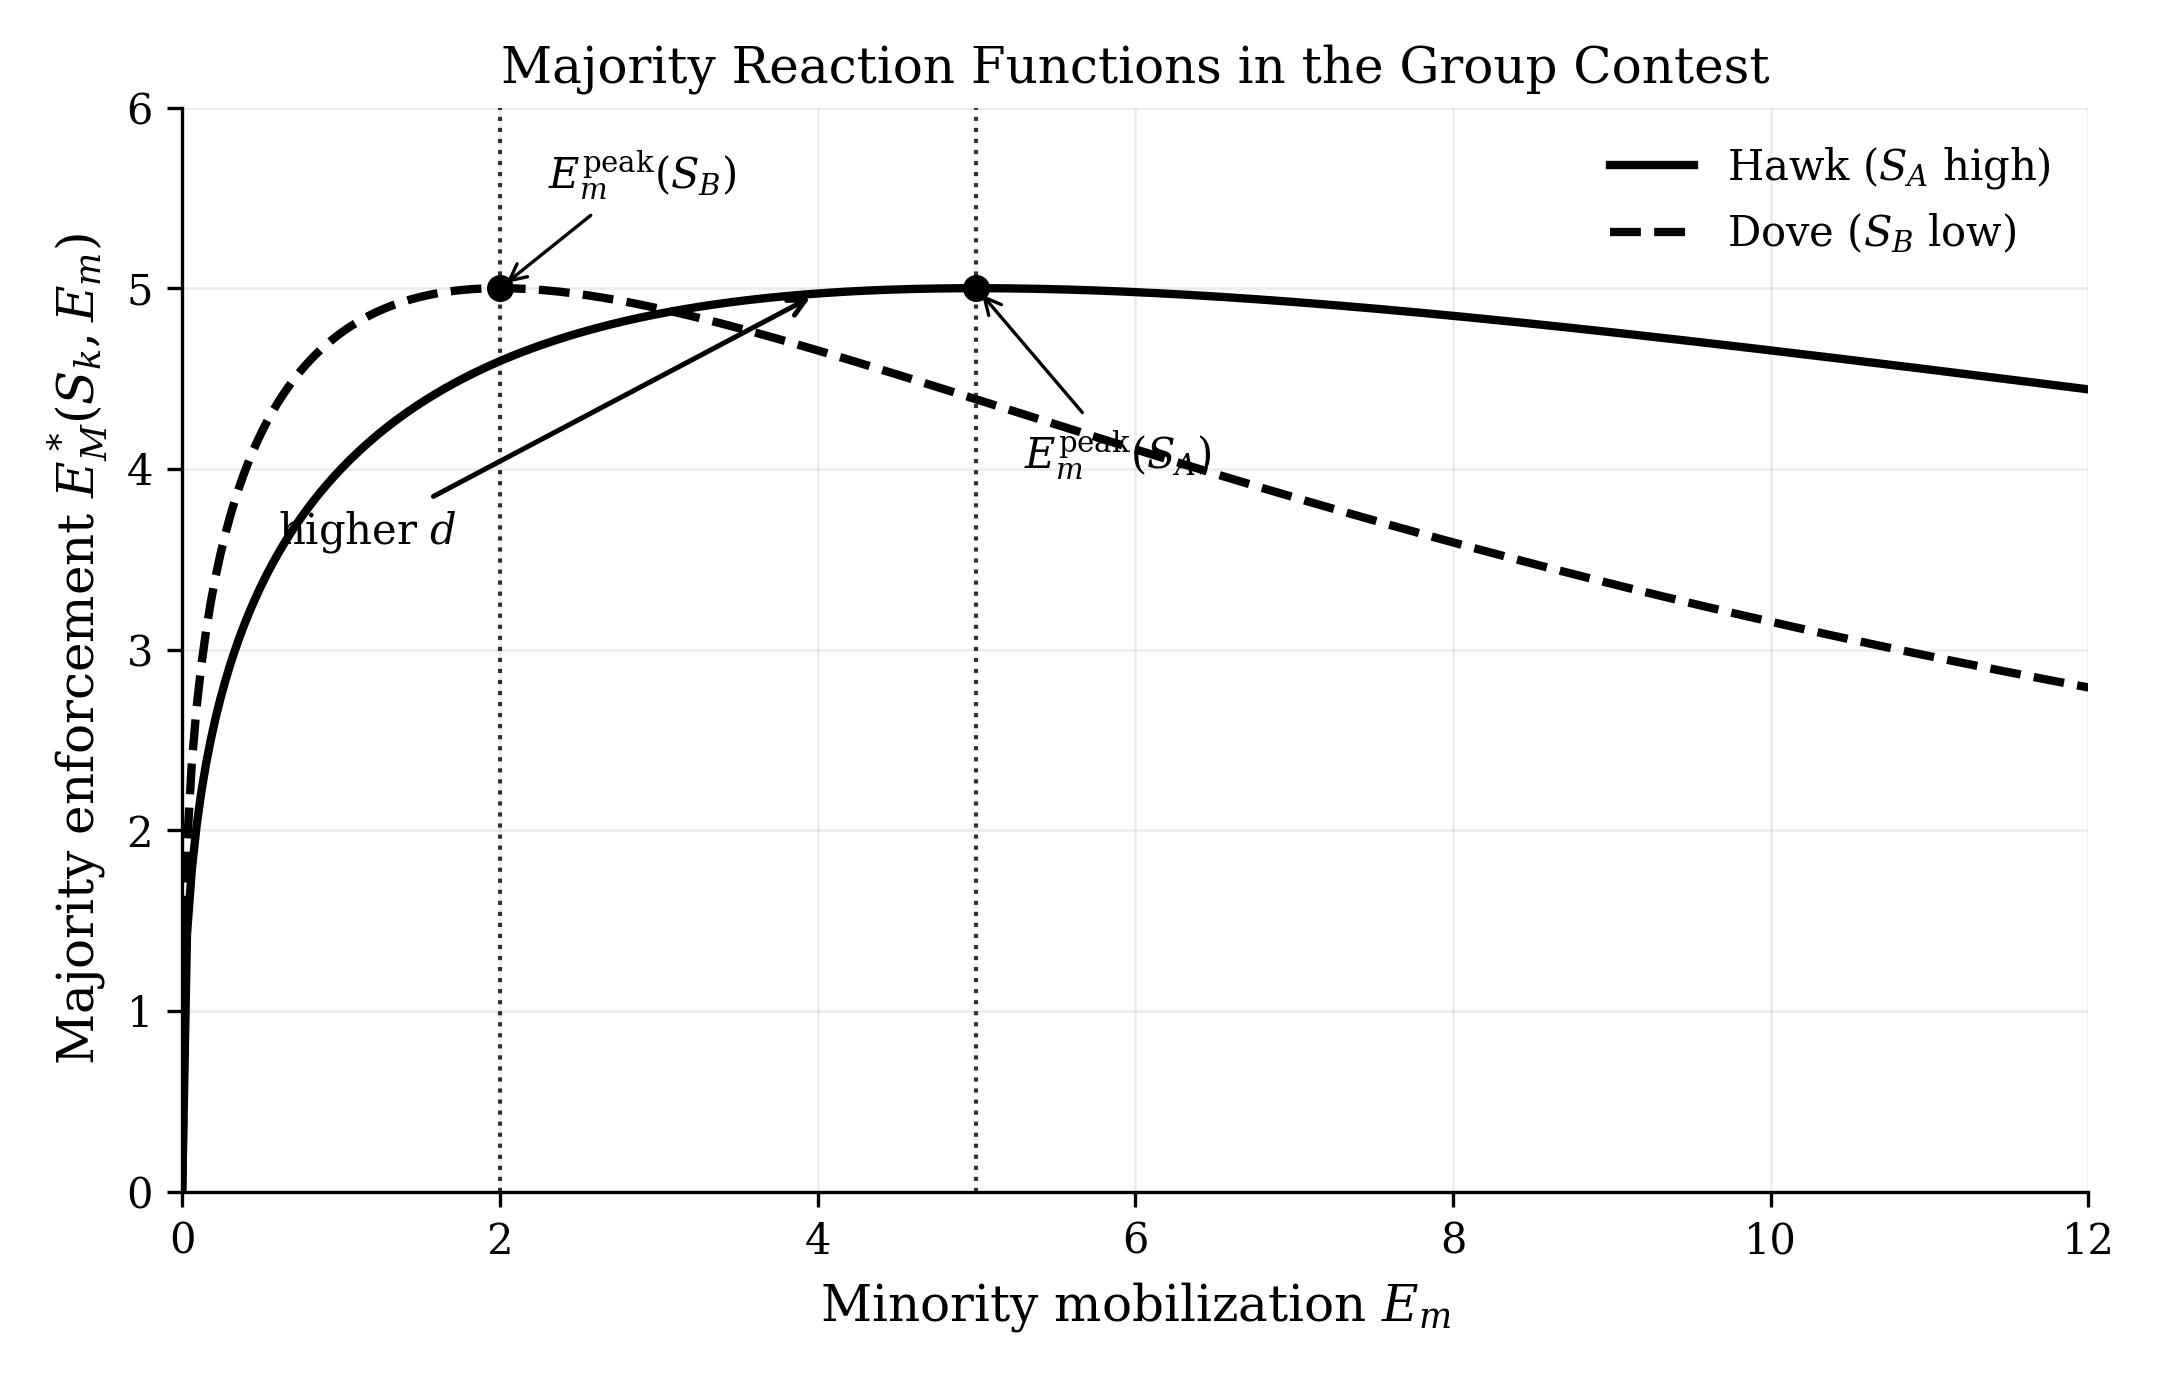
\includegraphics[width=0.92\textwidth]{figures/functions/fig_reaction_functions.jpg}
    \caption{\normalsize\bf Majority reaction functions and strategic complements/substitutes.}
    
    \floatfoot*{\footnotesize\textit{Notes}: The figure plots the equilibrium response $E_M^*(S_k,E_m)$ from \autoref{eq:EM_star} as a function of $E_m$, for two technology levels: a high-capacity Hawk ($S_A$) and a low-capacity Dove ($S_B$). Each curve is single-peaked at $E_m^{\mathrm{peak}}(S_k)$ from Lemma \autoref{lem:reaction_invertedU}. For $E_m<E_m^{\mathrm{peak}}(S_k)$, enforcement and opposition mobilization are strategic complements ($\partial E_M^*/\partial E_m>0$); for $E_m>E_m^{\mathrm{peak}}(S_k)$ they are strategic substitutes ($\partial E_M^*/\partial E_m<0$). The arrow illustrates how a more provocative symbolic policy $d$ raises $E_m(d)$ and thereby moves the economy along the high-$S_k$ reaction curve, activating Majority enforcement. Illustration uses $(N_M,\Lambda,S_A,S_B)=(100,1,1.0,0.4)$.}
    \label{fig:reaction_functions}
\end{figure}

\subsubsection{The inefficiency of the contest: rent dissipation under biased design}
Contest theory often measures the resource cost of conflict by the sum of equilibrium efforts (rent dissipation). In my environment, the incumbent's symbolic policy is the primitive ``design'' instrument that determines the contest intensity by shifting $E_m(d)$.

\begin{definition}[\textbf{Rent dissipation}] \label{def:rent_dissipation}
For an incumbent with technology $S_k$, define total rent dissipation under symbolic policy $d$ as
\begin{equation} \label{eq:RD}
RD(d,S_k)\equiv E_M^*\big(S_k,E_m(d)\big)+E_m(d)=E_M^*\big(S_k,\gamma d^{\sigma}\big)+\gamma d^{\sigma}.
\end{equation}
\end{definition}

\begin{proposition}[\textbf{Rent dissipation and biased contest design}] \label{prop:rent_dissipation}
For any $S_k>0$, rent dissipation satisfies $RD(0,S_k)=0$ and $RD(d,S_k)>0$ for all $d>0$. Moreover, the politically optimal symbolic policy generically features strictly positive dissipation: in any equilibrium in which the incumbent chooses $d_k^*>0$, the realized contest dissipates resources $RD(d_k^*,S_k)>0$.
Whenever symbolic policy induces a non-trivial threat, equilibrium mobilization generates rent dissipation through both opposition effort and enforcement.
\end{proposition}

\begin{proof}
Since $E_m(0)=0$ by \autoref{eq:reaction}, Lemma \autoref{lem:contest_equilibrium} implies $E_M^*(S_k,0)=0$ and hence $RD(0,S_k)=0$. If $d>0$, then $E_m(d)=\gamma d^{\sigma}>0$, and Lemma \autoref{lem:contest_equilibrium} implies $E_M^*(S_k,E_m(d))>0$. Therefore $RD(d,S_k)>0$ for all $d>0$.

The final statement follows immediately: if an incumbent chooses $d_k^*>0$ in equilibrium, then the induced dissipation is $RD(d_k^*,S_k)>0$ by the preceding argument. In particular, combining this observation with Proposition \autoref{prop:provocation} implies that strategic provocation (``arming the enemy'') in equilibrium is necessarily accompanied by strictly positive rent dissipation.
\end{proof}

Proposition \autoref{prop:rent_dissipation} records that any equilibrium with $d_k^*>0$ necessarily features positive rent dissipation, because $d$ induces $E_m(d)>0$ and triggers $E_M^*(S_k,E_m(d))>0$. In this sense, symbolic policy acts as a biased contest-design instrument that shifts political competition toward security at the cost of real resource waste.

\begin{figure}[t]
    \centering
    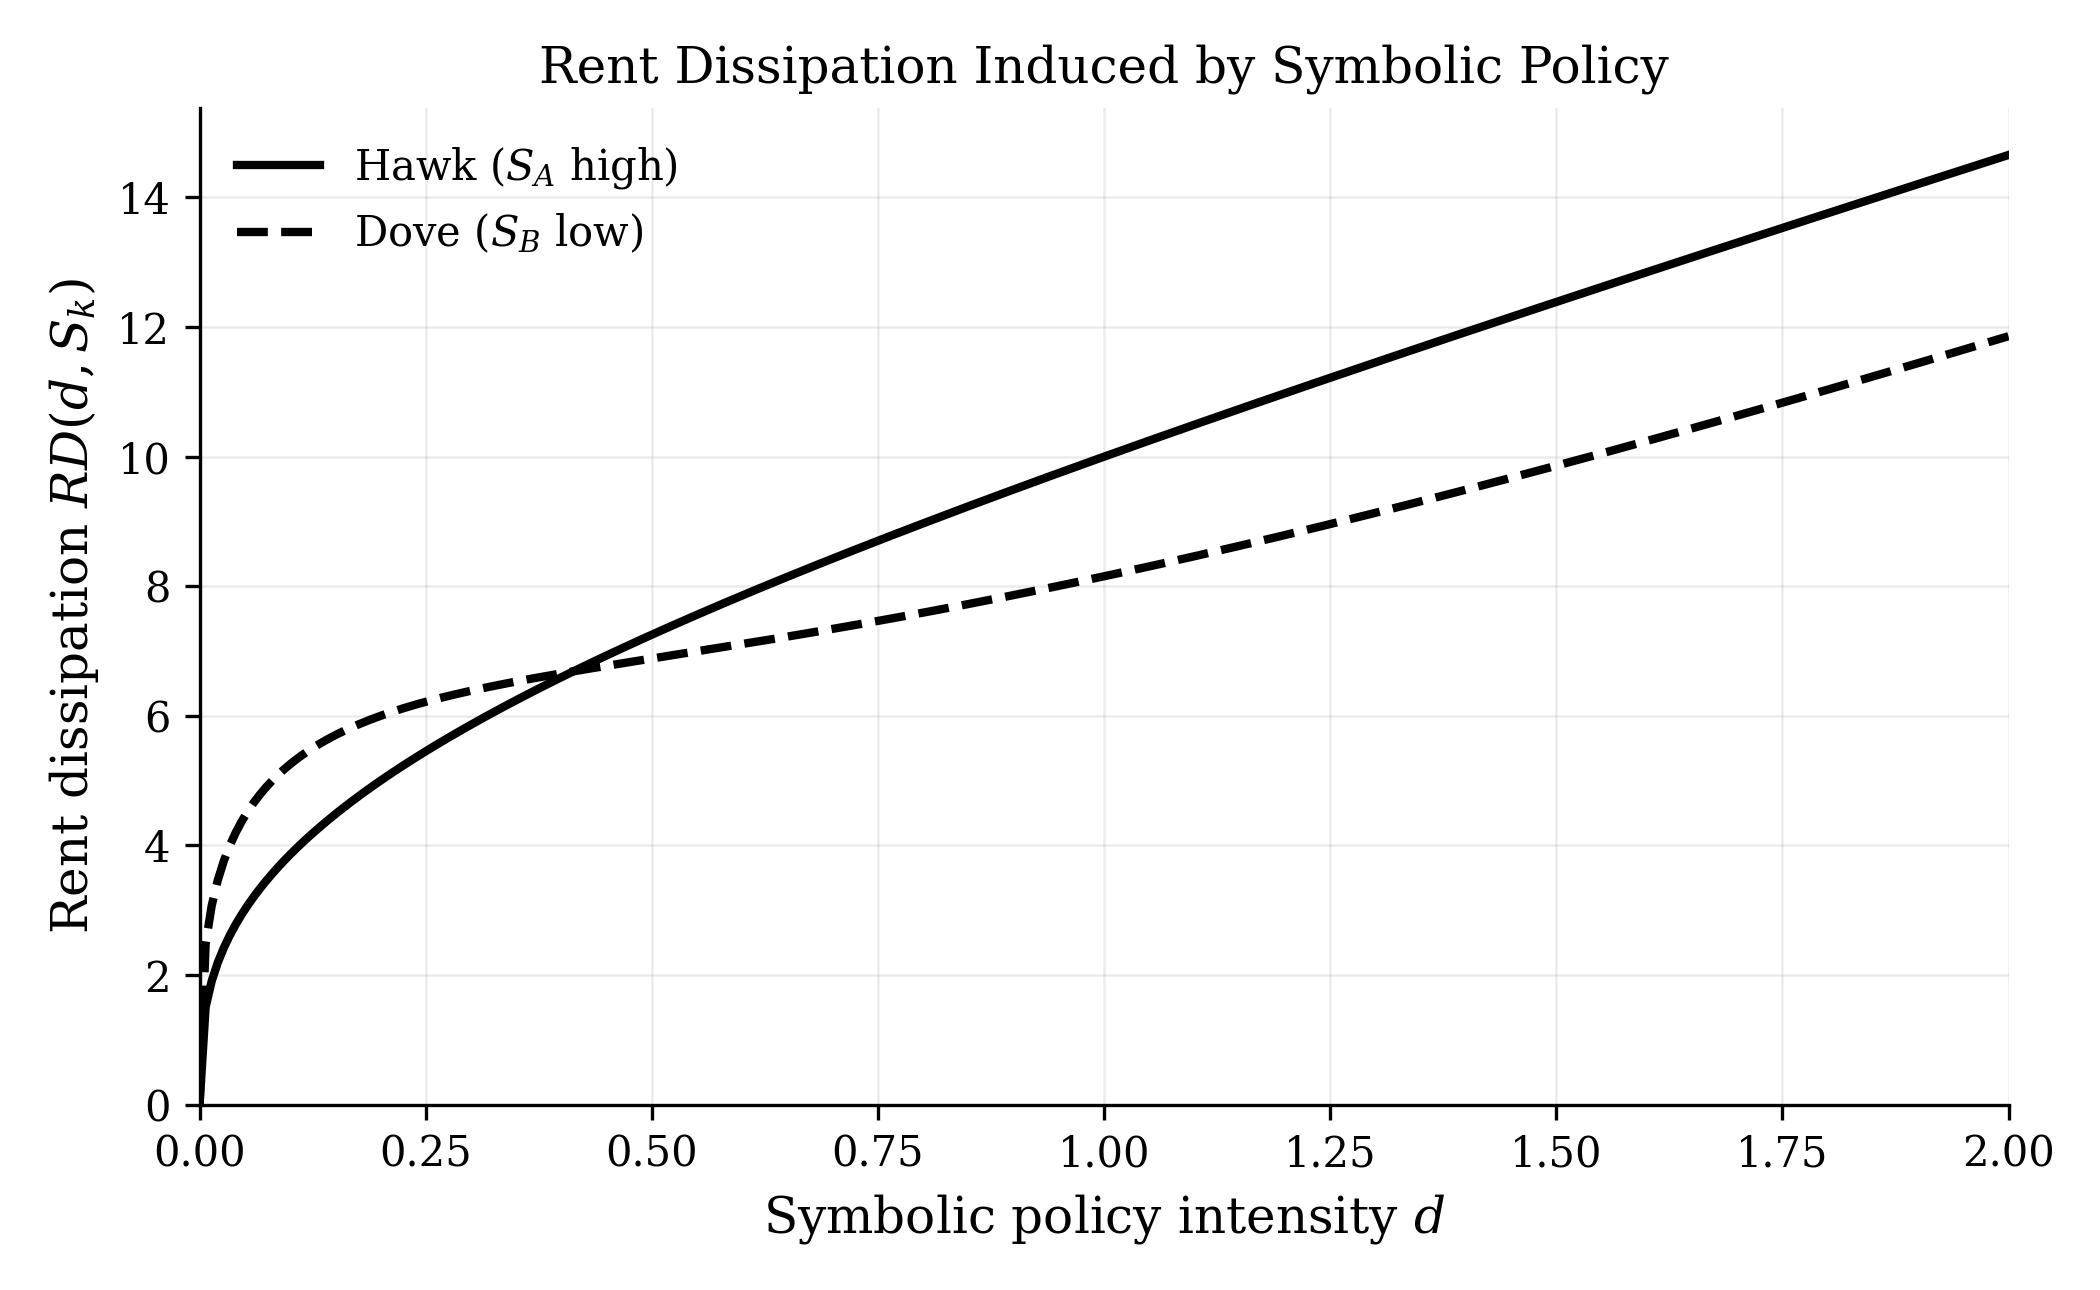
\includegraphics[width=0.88\textwidth]{figures/functions/fig_rent_dissipation.jpg}
    \caption{\normalsize\bf Rent dissipation under symbolic policy.}
    
    \floatfoot*{\footnotesize\textit{Notes}: The figure plots $RD(d,S_k)$ from \autoref{eq:RD} as a function of symbolic policy intensity $d$, for two levels of state capacity. Symbolic policy induces positive minority mobilization, $E_m(d)>0$, which generates a contest and leads to real resource dissipation through both minority mobilization and majority enforcement. Unlike the neutral contest designer in standard contest models (e.g., \citet{barut1998symmetric}), the political incumbent may optimally choose a strictly positive $d$, and hence positive dissipation, because conflict increases the security premium in elections. Parameters are $(N_M,\Lambda,\gamma,\sigma,S_A,S_B)=(100,1,5,1,1.0,0.2)$.}
\end{figure}

Taken together, by choosing $d_k$, the incumbent selects the threat environment $E_m(d_k)$ and thereby manipulates the equilibrium mapping from security competence $S_k$ into realized security $\Pi_k^*(d_k;S_k)$. This mechanism is central to the political economy analysis below.


\section{Voter Preferences and Electoral Competition}

Preferences in the Majority electorate are characterized by heterogeneity. Voter $i$ derives utility from a weighted combination of physical security and economic consumption, augmented by an idiosyncratic partisan bias. The per-period utility from electing Party $k\in\{A,B\}$ is:
\begin{equation} \label{eq:utility}
U_i^k = \lambda \Pi_k^*(d_k;S_k) + (1-\lambda) u(g_k) - \chi(d_k) + \xi_i,
\end{equation}
where $\lambda\in(0,1)$ is a fixed (exogenous) weight on security, and $\chi(d)$ is a convex cost of symbolic regulation borne by the Majority (economic disruption, administrative burden, or moderate-voter backlash), with $\chi'(d)>0$ and $\chi''(d)>0$. The term $\xi_i$ captures an idiosyncratic preference shock in favor of the Hawk, distributed according to a cumulative distribution function $\Phi(\cdot)$ with median zero (a normalization).

A citizen $i$ votes for Party $A$ if $U_i^A \geq U_i^B$. Substituting (\ref{eq:utility}), the indifference condition for the \textit{swing voter} $\hat{\xi}$ is:
\begin{equation} \label{eq:swing}
\hat{\xi} =
\underbrace{(1-\lambda) [u(g_B) - u(g_A)]}_{\text{Economic deficit}}
\;+\;
\underbrace{[\chi(d_A)-\chi(d_B)]}_{\text{Direct symbolic-policy cost}}
\;-\;
\underbrace{\lambda \Big(\Pi_A^*(d_A;S_A)-\Pi_B^*(d_B;S_B)\Big)}_{\text{Security premium}}.
\end{equation}
The first term captures the Hawk's economic deficit. The second term captures the direct cost of symbolic policy for the (swing) Majority electorate. The third term is the Security Premium. Party $A$ secures an electoral victory if the median voter prefers $A$, corresponding to $\Phi(-\hat{\xi}) > 1/2$.


\section{Baseline Analysis}

The political equilibrium is the subgame perfect equilibrium of the three-stage game described above. In the policy stage, the incumbent chooses symbolic policy $d_k$, taking $(S_k,g_k)$ as given party-type characteristics. In the contest stage, mobilization levels $E_m(d_k)$ and $E_M^*(S_k,E_m)$ are determined as in \autoref{eq:reaction}--\autoref{eq:Pi_star_d}. In the election stage, voters compare indirect utilities and the swing-voter threshold $\hat{\xi}$ in \autoref{eq:swing} pins down the re-election probability.

We first characterize the voting behavior of the Majority. A citizen $i$ votes for Party $A$ if $U_i^A \geq U_i^B$. Substituting the utility function from (\ref{eq:utility}) yields the swing-voter threshold $\hat{\xi}$ in \autoref{eq:swing}. Party $A$ secures an electoral victory if the median voter prefers $A$, which corresponds to $\Phi(-\hat{\xi}) > 1/2$. The incumbent's objective is therefore to maximize the vote share by manipulating $\hat{\xi}$.

The central mechanism of the model relies on the interaction between opposition strength and the collective action problem. Holding fixed the threat level $E_m$ faced at the election, define the \textit{Security Premium} as the difference in equilibrium security provided by the Hawk versus the Dove,
\begin{equation} \label{eq:security_premium}
\Delta \Pi(E_m)\;\equiv\;\Pi_A^*(S_A,E_m)-\Pi_B^*(S_B,E_m),
\end{equation}
where $\Pi_k^*(S_k,E_m)$ is defined in \autoref{eq:Pi_star}.

\begin{lemma}[\textbf{Comparative Advantage in Conflict}] \label{lem:advantage}
Suppose $S_A>S_B$. The Security Premium $\Delta \Pi(E_m)$ satisfies $\Delta \Pi(0)=0$, $\Delta \Pi(E_m)>0$ for all $E_m>0$, and $\lim_{E_m\uparrow\infty}\Delta\Pi(E_m)=0$. Moreover, there exists $\overline{E}>0$ such that $\Delta \Pi(E_m)$ is strictly increasing on $[0,\overline{E}]$.
The Hawk's security advantage is absent in peace, strictly positive under any non-trivial opposition mobilization, and vanishes again under extreme mobilization; moreover, it increases with $E_m$ for sufficiently small threats.
\end{lemma}

\begin{proof}
The boundary conditions follow from Lemma \autoref{lem:contest_equilibrium}. In particular, $\lim_{E_m\downarrow 0}\Pi_k^*(S_k,E_m)=1$ for any $S_k>0$, so $\Delta\Pi(0)=0$. Moreover, $\Pi_k^*(S_k,E_m)$ is strictly increasing in $S_k$ for any $E_m>0$, so $\Delta\Pi(E_m)>0$ whenever $E_m>0$. Finally, $\lim_{E_m\uparrow\infty}\Pi_k^*(S_k,E_m)=0$, so $\lim_{E_m\uparrow\infty}\Delta\Pi(E_m)=0$.

To show that $\Delta\Pi$ is strictly increasing near $E_m=0$, write equilibrium security as $\Pi_k^*(S_k,E_m)=r_k/(r_k+1)$, where $r_k\equiv Z_k/E_m$ and $Z_k$ satisfies \autoref{eq:Z_star}. Dividing \autoref{eq:Z_star} by $E_m^3$ yields
\begin{equation} \label{eq:r_equation}
r_k(r_k+1)^2=\frac{N_M\Lambda S_k^2}{E_m^2}.
\end{equation}
As $E_m\downarrow 0$, the right-hand side of \autoref{eq:r_equation} diverges to $+\infty$, so $r_k\to+\infty$. Using $r_k(r_k+1)^2=r_k^3(1+o(1))$ as $r_k\to\infty$, \autoref{eq:r_equation} implies $r_k=(N_M\Lambda)^{1/3}S_k^{2/3}E_m^{-2/3}(1+o(1))$. Therefore
\[
\Pi_k^*(S_k,E_m)=1-\frac{1}{r_k+1}=1-(N_M\Lambda)^{-1/3}S_k^{-2/3}E_m^{2/3}(1+o(1)).
\]
It follows that, as $E_m\downarrow 0$,
\[
\Delta\Pi(E_m)=(N_M\Lambda)^{-1/3}E_m^{2/3}\Big(S_B^{-2/3}-S_A^{-2/3}\Big)(1+o(1)),
\]
which is strictly increasing in $E_m$ for $E_m$ sufficiently small. Hence there exists $\overline{E}>0$ such that $\Delta\Pi$ is strictly increasing on $[0,\overline{E}]$.
\end{proof}

The Security Premium is therefore an indirect function of symbolic policy through the opposition's reaction, $\Delta\Pi(E_m(d))$. In the baseline electoral problem, the Hawk chooses symbolic regulation to trade off a larger Security Premium against the direct electoral cost $\chi(d)$.

\begin{proposition}[\textbf{Strategic Provocation and an Economic-Deficit Cutoff}] \label{prop:provocation}
Assume the Dove's symbolic policy is fixed at $d_B=0$, $\chi$ is continuous, $\chi(0)=0$, and $\lim_{d\to\infty}\chi(d)=\infty$. Let the Hawk's economic disadvantage be $\Delta u \equiv u(g_B)-u(g_A)>0$. In the Hawk's static policy problem, any winning choice $d_A^*$ satisfies $d_A^*>0$ and hence $E_m(d_A^*)>0$. Moreover, define the cutoff
\begin{equation} \label{eq:delta_u_bar}
\overline{\Delta u}\;\equiv\;\frac{1}{1-\lambda}\max_{d\ge 0}\Big\{\lambda \Delta \Pi(E_m(d))-\chi(d)\Big\}.
\end{equation}
A Hawk victory is feasible if and only if $\Delta u \le \overline{\Delta u}$.
To win despite an economic deficit, the Hawk must choose strictly positive symbolic policy to induce opposition mobilization and activate a Security Premium, and there is a finite bound on how large a deficit this channel can offset.
\end{proposition}
\begin{proof}
Fix $d_B=0$. Since Party $A$ maximizes its vote share, it equivalently minimizes the swing-voter threshold $\hat{\xi}$ in \autoref{eq:swing}. Under $\chi(0)=0$ and $d_B=0$, the threshold is
\begin{equation} \label{eq:xi_hat_d}
\hat{\xi}(d)\;=\;(1-\lambda)\Delta u+\chi(d)-\lambda\Delta\Pi(E_m(d)).
\end{equation}
Since Party $A$'s vote share is $\Phi(-\hat{\xi}(d))$ and $\Phi$ is increasing, maximizing votes is equivalent to minimizing $\hat{\xi}(d)$. In \autoref{eq:xi_hat_d}, the economic disadvantage $(1-\lambda)\Delta u$ does not vary with $d$, so the policy stage is a choice of $d$ that balances two policy-sensitive forces: the direct electoral cost $\chi(d)$ borne by the Majority, and the security premium $\Delta\Pi(E_m(d))$ created by the opposition response to symbolic policy. Party $A$ therefore chooses $d$ to maximize the net electoral return
\begin{equation} \label{eq:provocation_objective}
F(d)\;\equiv\;\lambda\Delta\Pi(E_m(d))-\chi(d).
\end{equation}
Because $0\le \Delta\Pi(E_m(d))\le 1$ and $\chi(d)\to\infty$, the continuous objective $F$ attains a maximizer $d_A^*\in[0,\infty)$. If $F$ is differentiable on $(0,\infty)$, any interior optimum satisfies the first-order condition $\lambda \Delta\Pi'(E_m(d_A^*))E_m'(d_A^*)=\chi'(d_A^*)$.
Because $E_m(0)=0$ by \autoref{eq:reaction}, and because in the absence of opposition mobilization ($E_m=0$) both parties deliver full dominance (so $\Pi_A=\Pi_B=1$), it follows that $\Delta\Pi(E_m(0))=0$ and hence $F(0)=0$.

If the Hawk wins, then the median voter weakly prefers $A$, i.e., $\hat{\xi}(d_A^*)\le 0$. By \autoref{eq:xi_hat_d}, this requires $F(d_A^*)\ge (1-\lambda)\Delta u>0$. Since $F(0)=0$, it follows that $d_A^*\neq 0$, so any winning choice must satisfy $d_A^*>0$ and therefore $E_m(d_A^*)>0$.

For the cutoff, note that the Hawk wins if and only if there exists a feasible $d\ge 0$ such that $(1-\lambda)\Delta u\le \lambda \Delta \Pi(E_m(d))-\chi(d)$. Maximizing the right-hand side over $d$ yields \autoref{eq:delta_u_bar}. If $\Delta u \le \overline{\Delta u}$, then a winning $d$ exists; if $\Delta u > \overline{\Delta u}$, then no symbolic policy can offset the Hawk's economic deficit.
\end{proof}

Proposition \autoref{prop:provocation} shows identity politics as a subtitute for competence and its limit. The Hawk is structurally disadvantaged on economic performance, so it cannot win by competing on the public good dimension. In a peaceful environment, this disadvantage is critical in elections because the underlying contest is not active. When $E_m=0$, the economy is under peaceful environment, so security premium of the Hawk is diminished. Once their economic incompetence is revealed, the Hawk loses the election. To survive, the Hawk starts provocation. By choosing $d_A^*>0$, the Hawk manufactures a visible threat and triggers Minority mobilization ($E_m>0$). This raises the importance in the security dimension in the contest. The security technology of contesters are electorally relevant. 

Term $\bar{\Delta U}$ captures how much voters will sacrifice in economic payoff for identity security. When $\Delta U>\bar{\Delta U}$, the electorate's tolerance for economic benefit breaks. Restoring consumption dominates any additional security advantage the Hawk can create with identity contestation. Under these mechanisms, a significant negative economic shock could moderate identity politics in an electorial economy.

\section{Dynamic Extension: Myopia, Forgetting, and Regime Switching}

This section develops a parsimonious dynamic extension that delivers political-economy cycles, alternating high-$d$/low-$g$ and low-$d$/high-$g$ regimes, without allowing the preference weight on security $\lambda$ to vary over time. The key ingredients are (i) aggregate shocks that are imperfectly observed, (ii) retrospective (myopic) electoral accountability, and (iii) the regime-dependence of conflict production through $S_k$ and the induced equilibrium mobilization $E_M^*(S_k,E_m)$.

\subsection{Aggregate shocks and noisy performance}
Time is discrete, $t=0,1,2,\dots$, and an election takes place each period. Let $\theta_t$ denote an aggregate economic state and $\omega_t$ an aggregate threat state. For expositional simplicity, take party characteristics $(S_k,g_k,d_k)$ as stationary over time, with $g_B>g_A$ and $d_A>d_B$.

Under a candidate party $k\in\{A,B\}$, the realized economic payoff is
\begin{equation}
c_{k,t} = \theta_t g_k,
\end{equation}
and minority mobilization is
\begin{equation}
E_{m,t}(k)=\omega_t \gamma d_k^{\sigma}.
\end{equation}
Given $(S_k,E_{m,t}(k))$, Majority mobilization is $E_{M,t}^*(S_k,E_{m,t}(k))$, and security is $\Pi_{k,t}=\Pi_k(E_{M,t}^*,E_{m,t}(k))$ as in \autoref{eq:CSF}.

Voters do not observe $(\theta_t,\omega_t)$ nor the counterfactual outcomes under the challenger. Instead, they observe noisy performance signals of consumption and disorder under the incumbent regime $k_t$:
\begin{equation}
\tilde{c}_t = c_{k_t,t} + \varepsilon_t^c, \qquad \tilde{v}_t = \big(1-\Pi_{k_t,t}\big) + \varepsilon_t^v,
\end{equation}
where $\tilde{v}_t$ is a reduced-form measure of observable street disorder/violence. Importantly, because $\Pi_{k,t}$ depends on $S_k$ and the endogenous response $E_{M,t}^*(S_k,E_m)$, the same underlying threat $\omega_t$ can generate very different observed disorder across regimes.

\subsection{Forward-looking voting and the conflict trap}
Depending on voter patience, the dynamic environment admits two qualitatively distinct equilibrium paths. When voters are forward-looking, regime choice is governed by the discounted value of future security capacity.

\begin{proposition}[\textbf{Conflict Trap}] \label{prop:trap}
Assume voters are forward-looking with discount factor $\delta\in[0,1)$ and form rational expectations about the future evolution of $(\theta_t,\omega_t)$ under each regime. There exists a critical patience threshold $\bar{\delta}\in(0,1)$ such that for all $\delta>\bar{\delta}$, the Hawk regime is an absorbing state in a stationary political equilibrium. In particular, conditional on a Hawk incumbent, the electorate retains the Hawk even after the most adverse economic realizations $\theta_t=\underline{\theta}$ in order to avoid the discrete reduction in security capacity associated with switching from $S_A$ to $S_B$.
Sufficiently patient voters tolerate even severe short-run economic losses to avoid a persistent drop in future security capacity.
\end{proposition}

\begin{proof}
Fix an incumbent Hawk regime and suppress the idiosyncratic taste term $\xi_i$ by considering the median voter (normalized to have $\xi_i=0$). Let
\begin{equation}
\Omega(\theta,\omega)\;\equiv\;\lambda\Big(\Pi_A^*(S_A,\omega\gamma d_A^{\sigma})-\Pi_B^*(S_B,\omega\gamma d_B^{\sigma})\Big)-(1-\lambda)\Big(u(\theta g_B)-u(\theta g_A)\Big)-\big[\chi(d_A)-\chi(d_B)\big]
\end{equation}
denote the one-period net advantage of the Hawk relative to the Dove in state $(\theta,\omega)$. Consider the worst economic realization $\underline{\theta}$ and assume (as in the proposition) that it constitutes the most unfavorable state for the Hawk's re-election incentive.

To isolate the role of patience, consider a transitory recession at date $t$ with $\theta_t=\underline{\theta}$, followed by reversion from $t+1$ onward to a stationary environment. In that continuation environment, the discrete gap in security capacity ($S_A>S_B$) implies that the expected per-period net advantage of the Hawk is strictly positive:
\begin{equation} \label{eq:omega_bar}
\overline{\Omega}\;\equiv\;\mathbb{E}\big[\Omega(\theta,\omega)\mid t+1\text{ onward}\big]\;>\;0.
\end{equation}
Let $\underline{\Omega}\equiv \mathbb{E}\big[\Omega(\underline{\theta},\omega_t)\big]$ denote the expected one-period net advantage during the recession. The forward-looking value difference between retaining the Hawk and switching regimes at date $t$ can then be expressed (via the Bellman equations under stationarity from $t+1$ onward) as
\begin{equation}
\Delta V_t \;=\; \underline{\Omega} + \sum_{\tau=t+1}^{\infty}\delta^{\tau-t}\overline{\Omega}
\;=\; \underline{\Omega} + \frac{\delta}{1-\delta}\overline{\Omega}.
\end{equation}
The function $\Delta V_t(\delta)$ is continuous and strictly increasing on $[0,1)$. Moreover, $\lim_{\delta\uparrow 1}\Delta V_t(\delta)=+\infty$ by \autoref{eq:omega_bar}. Hence there exists a cutoff $\bar{\delta}\in(0,1)$ such that $\Delta V_t(\delta)\ge 0$ for all $\delta\ge \bar{\delta}$. For $\delta>\bar{\delta}$ the median voter weakly prefers to retain the Hawk even when $\theta_t=\underline{\theta}$. Since $\underline{\theta}$ is the most adverse economic realization, the Hawk is retained in every state, implying that the Hawk regime is absorbing in a stationary equilibrium.
\end{proof}

\autoref{prop:trap} demonstrates how patience of voters interacts with accountability. Voters internalize regime switching from Hawk to Dove put them into weaker technologies of identity protection. A weak $S$ entails weaker ability of the majority to coordinate under future threats of minority. When $\delta$ is sufficient high, the discounted value of avioding future risks dominates even the worst contemporaneous economi shock $\underline{\theta}$. Current electorial punishment for economic underperformance of the Hawk fades because of voter's future concerns over identity security. This mechanism captures why identity-fragmented societies be locked into a conflict trap in which the Hawk survive indefinitely long despite worse economic management.

\subsection{Myopic voting and regime transitions}
Let per-period utility be given by (\ref{eq:utility}). A forward-looking voter with discount factor $\delta\in[0,1)$ evaluates parties by lifetime value. The special case $\delta\to 0$ corresponds to purely retrospective (myopic) voting: the electorate selects the party that maximizes perceived one-period utility based on the current performance signals $(\tilde{c}_t,\tilde{v}_t)$.

To connect the dynamic environment to the static swing-voter logic, define the perceived one-period Hawk-selection condition
\begin{equation} \label{eq:dyn_switch}
\lambda\Big(\mathbb{E}_t[\Pi_{A,t}]-\mathbb{E}_t[\Pi_{B,t}]\Big)\;\ge\;(1-\lambda)\Big(\mathbb{E}_t[u(\theta_t g_B)]-\mathbb{E}_t[u(\theta_t g_A)]\Big)+\big[\chi(d_A)-\chi(d_B)\big],
\end{equation}
which is the dynamic analogue of \autoref{eq:swing}.

\begin{proposition}[\textbf{Political Cycles}] \label{prop:cycles}
Assume voters are myopic ($\delta=0$), and $(\theta_t,\omega_t)$ are stochastic with full support on $[\underline{\theta},\overline{\theta}]\times[\underline{\omega},\overline{\omega}]$. Suppose (i) the posterior expectations entering \autoref{eq:dyn_switch} are monotone in the underlying states,\footnote{For instance, a natural sufficient condition is that the signal structure $(\tilde{c}_t,\tilde{v}_t)$ satisfies a monotone likelihood ratio property so that $\mathbb{E}_t[\theta_t]$ and $\mathbb{E}_t[\omega_t]$ are monotone in the realized signals.} (ii) for $g_B>g_A$, the function $\theta \mapsto u(\theta g_B)-u(\theta g_A)$ is strictly decreasing on $[\underline{\theta},\overline{\theta}]$, and (iii) the Security Premium is increasing in minority mobilization over the policy-relevant domain (Lemma \autoref{lem:advantage}). Assume further that the myopic election rule selects different parties in different states (i.e., there exist $(\theta,\omega)$ and $(\theta',\omega')$ in the support such that \autoref{eq:dyn_switch} holds in one and fails in the other). Then the political equilibrium exhibits recurrent regime switching. In particular:
\begin{enumerate}[label=(\roman*)]
    \item (\emph{Hawk $\rightarrow$ Dove}) Conditional on a Hawk incumbent, the probability of a regime change is strictly decreasing in $\theta_t$.
    \item (\emph{Dove $\rightarrow$ Hawk}) Conditional on a Dove incumbent, the probability of a regime change is strictly increasing in the threat environment $\omega_t$, the minority's structural mobilization potential $\gamma$, and the security weight $\lambda$.
\end{enumerate}
Myopic retrospective voting makes regime choice track current conditions: adverse economics push the electorate toward the Dove, while high perceived threat pushes it toward the Hawk.
\end{proposition}

\begin{proof}
Under myopic voting ($\delta=0$), the median voter elects the Hawk at date $t$ if and only if \autoref{eq:dyn_switch} holds. Define the net advantage
\begin{equation}
\Omega_t \;\equiv\; \lambda\Big(\mathbb{E}_t[\Pi_{A,t}]-\mathbb{E}_t[\Pi_{B,t}]\Big)-(1-\lambda)\Big(\mathbb{E}_t[u(\theta_t g_B)]-\mathbb{E}_t[u(\theta_t g_A)]\Big)-\big[\chi(d_A)-\chi(d_B)\big],
\end{equation}
so the Hawk is elected if and only if $\Omega_t\ge 0$.

For part (i), note that for $g_B>g_A$,
\begin{equation}
\frac{\partial}{\partial \theta}\Big(u(\theta g_B)-u(\theta g_A)\Big)=g_Bu'(\theta g_B)-g_Au'(\theta g_A),
\end{equation}
so assumption (ii) is equivalent to $g_Bu'(\theta g_B)-g_Au'(\theta g_A)<0$ on $[\underline{\theta},\overline{\theta}]$.\footnote{A common sufficient condition is CRRA utility $u(c)=c^{1-\rho}/(1-\rho)$ with $\rho>1$, in which case $g_Bu'(\theta g_B)-g_Au'(\theta g_A)=\theta^{-\rho}\big(g_B^{1-\rho}-g_A^{1-\rho}\big)<0$ for all $\theta>0$.} Combining this with assumption (i), a lower realization of $\theta_t$ strictly increases the perceived economic advantage of the Dove and therefore strictly decreases $\Omega_t$.

Moreover, $\Omega_t$ is continuous in $(\theta_t,\omega_t)$ (given continuity of $u$ and monotone posteriors), and by hypothesis there exist states in which $\Omega_t\ge 0$ and states in which $\Omega_t<0$. Fix any $\omega\in[\underline{\omega},\overline{\omega}]$ and hold $\omega_t=\omega$. The previous argument implies that $\Omega_t$ is strictly increasing in $\theta_t$ on $[\underline{\theta},\overline{\theta}]$. Hence the intermediate value theorem yields a cutoff $\theta^*(\omega)\in(\underline{\theta},\overline{\theta})$ such that the myopic electorate selects the Hawk if and only if $\theta_t\ge \theta^*(\omega_t)$. Therefore, conditional on a Hawk incumbent, the Hawk $\rightarrow$ Dove transition event $\{\Omega_t<0\}$ is equivalent to $\{\theta_t<\theta^*(\omega_t)\}$, which becomes (weakly) more likely under more adverse economic realizations.

For part (ii), note that minority mobilization satisfies $E_{m,t}(k)=\omega_t\gamma d_k^{\sigma}$, so higher $\omega_t$ or higher $\gamma$ increases the threat faced under either candidate platform. By Lemma \autoref{lem:advantage} (over the relevant domain), the perceived Security Premium $\mathbb{E}_t[\Pi_{A,t}-\Pi_{B,t}]$ is increasing in the threat level, so $\Omega_t$ is increasing in $\omega_t$ and $\gamma$. Moreover,
\begin{equation}
\frac{\partial \Omega_t}{\partial \lambda} = \Big(\mathbb{E}_t[\Pi_{A,t}]-\mathbb{E}_t[\Pi_{B,t}]\Big)+\Big(\mathbb{E}_t[u(\theta_t g_B)]-\mathbb{E}_t[u(\theta_t g_A)]\Big) > 0,
\end{equation}
so $\Omega_t$ is increasing in $\lambda$. Therefore the probability that $\Omega_t$ crosses zero in favor of the Hawk (a Dove $\rightarrow$ Hawk transition) is increasing in $\omega_t$, $\gamma$, and $\lambda$.

Finally, since the state process has full support and (by assumption) there exist states in which $\Omega_t\ge 0$ and states in which $\Omega_t<0$, both transitions occur with positive probability along the realized path, yielding recurrent regime switching.
\end{proof}

Myopic voting breaks the electoral trap by limiting voter's horizon to current signals. When a Hawk incumbent successfully suppress visible disorder, voters infer (contemporaneously) current environment is peaceful but fails to account for the peace is sustained by high security capacity by the Hawk party. Under this equilibrium, a sufficiently adverse economic realization triggers the electorate to vote for the Dove party to recover public goods provision in the economy. When the Dove is incumbent, lower capacity in identity security weakens Majority mobilization, reduces deterrence, and the safety equilibrium cannot be sustained. Identity threat from the Minority triggers a swing back to the Hawk to contain the potential disorder with cultural policies.

The resulting cycles can be read as over-correction as voters demand the dimension that is currently scarce. Economic prosperity is demanded in peaceful periods and security in identity is demanded in turbulent periods. The economy therefore oscillates between cycles of political control due to the presence of the minority.

\begin{corollary}[\textbf{The Paradox of Competence}] \label{cor:competence}
Under myopic voting ($\delta=0$), a first-order stochastic decrease in observed disorder under a Hawk incumbent (lower $\tilde{v}_t$) weakly decreases the perceived Security Premium in \autoref{eq:dyn_switch} and thereby weakly increases the probability of a Hawk defeat. Consequently, conditional on a Hawk incumbent, the hazard of regime change is decreasing in observed disorder.
A more successful Hawk can look less necessary in equilibrium: quieter streets shrink the perceived Security Premium and can increase turnover risk.
\end{corollary}

\begin{proof}
Under myopic voting, the Hawk is re-elected at date $t$ if and only if \autoref{eq:dyn_switch} holds, equivalently if $\Omega_t\ge 0$ where $\Omega_t$ is defined in the proof of Proposition \autoref{prop:cycles}. By assumption (i) in Proposition \autoref{prop:cycles} (and the monotone-likelihood-ratio sufficient condition in its footnote), a lower realization of the disorder signal $\tilde{v}_t$ weakly shifts posterior beliefs toward a lower threat environment and therefore weakly decreases the perceived Security Premium $\mathbb{E}_t[\Pi_{A,t}-\Pi_{B,t}]$.

Since $\Omega_t$ is increasing in $\mathbb{E}_t[\Pi_{A,t}-\Pi_{B,t}]$, a first-order stochastic decrease in $\tilde{v}_t$ induces a first-order stochastic decrease in $\Omega_t$ and hence weakly decreases $\mathbb{P}(\Omega_t\ge 0)$, the re-election probability of the Hawk. Equivalently, the probability of a regime change, $\mathbb{P}(\Omega_t<0)$, weakly increases when observed disorder is stochastically lower.
\end{proof}

Corollary \autoref{cor:competence} highlights an inference effect: under myopia, low observed disorder under the Hawk shifts beliefs toward a benign threat environment and reduces the perceived Security Premium, raising the probability of a Hawk defeat.

Together, Propositions \autoref{prop:trap} and \autoref{prop:cycles} show that the same micro-foundation, namely a biased incumbent manipulating a group contest to solve a collective action problem, can generate either long-run entrenchment or recurrent turnover. Patience makes the electorate internalize the durable loss of security capacity from regime change, producing an absorbing Hawk equilibrium. Myopia makes voters treat security as a contemporaneous outcome, opening the door to regime switching driven by noisy shocks and retrospective accountability.



\clearpage

\newpage
%=======================================================================================================%
\singlespacing
\footnotesize
\bibliographystyle{aer}

\begingroup
% \raggedright
\bibliography{ref}
\endgroup

\end{document}
